% !TeX program = pdflatex
% !TeX encoding = UTF-8
\documentclass[journal]{IEEEtran}
\usepackage{amsmath}
\usepackage{float}
\usepackage{amsfonts}
\usepackage{amssymb}
\usepackage{bm}
\usepackage{graphicx}
\usepackage{booktabs}
\usepackage{placeins}
\usepackage{xurl}
\usepackage{balance}
\usepackage{tikz}
\usetikzlibrary{arrows.meta,positioning}
\usepackage[hidelinks]{hyperref}

\hypersetup{
  pdftitle={On Using Fisher Information to Evaluate the Preservation of Spatial Discriminability in HRTF Upsampling},
  pdfauthor={Dominic Bassett, Matthew Cheshire, and Samuel Smith},
  pdfsubject={Evaluation of spatial discriminability preservation in HRTF upsampling},
  pdfkeywords={Fisher information, HRTF, spatial audio, spatial discriminability, upsampling}
}

\setlength{\textfloatsep}{5pt plus 1pt minus 2pt}
\setlength{\floatsep}{5pt plus 1pt minus 2pt}
\setlength{\intextsep}{5pt plus 1pt minus 2pt}
\setlength{\abovecaptionskip}{3pt plus 1pt minus 1pt}
\setlength{\belowcaptionskip}{0pt}

\title{On Using Fisher Information to Evaluate the Preservation of Spatial Discriminability in HRTF Upsampling}
\author{Dominic Bassett, Matthew Cheshire, and Samuel Smith%
\thanks{Dominic Bassett, Matthew Cheshire, and Samuel Smith are with Birmingham City University, Birmingham, U.K.}}

\begin{document}

\maketitle

\begin{abstract}
HRTF upsampling is typically evaluated using signal-domain reconstruction errors and localisation-model summaries, neither of which directly measures the preservation of local spatial discriminability. We introduce an evaluation method based on Fisher information on the sphere of source directions. Spatial gradients of positive spectral-gradient, interaural level-difference, and interaural time-difference features form a bivariate Fisher information tensor, whose inverse gives the Cramér--Rao bound on the covariance of an unbiased local angular estimator. Reference and reconstructed tensors are compared using the affine-invariant Riemannian metric, measuring changes in the scale, anisotropy, and orientation of local spatial discrimination ellipses. We evaluate the method on a 41-subject SONICOM cohort under four sparse-grid retention conditions. The comparison includes SUpDEq-based interpolation, RANF, and FSP-AE, and reports Fisher-tensor error alongside log-spectral distance and Bayesian localisation metrics. RANF achieves the lowest log-spectral distance across all conditions and the lowest tensor error at the three sparsest grids; FSP-AE maintains stable tensor errors despite higher log-spectral distance. Projected \(\bm{d'=1}\) thresholds express selected tensors in angular units and show the expected increase in lateral threshold from frontal to lateral directions. The proposed evaluation therefore quantifies reconstruction errors in predicted local spatial discriminability that are not measured by signal fidelity or localisation summaries alone.
\end{abstract}

\begin{IEEEkeywords}
Fisher information, head-related transfer functions, information geometry,
spatial audio, spatial discriminability, upsampling.
\end{IEEEkeywords}

\section{Introduction and Background}

Head-related transfer functions (HRTFs) encode the direction-dependent filtering imposed by the listener's head, torso, and pinnae. Dense individual HRTF measurements are expensive to obtain, so spatial upsampling may be used to reconstruct a dense directional field from a sparse set of measured directions. Upsampling methods are usually evaluated with log-spectral distance (LSD), interaural level-difference error, interaural time-difference error, and localisation-model summaries. These quantities measure signal fidelity or predicted pointing performance, but they do not directly ask whether the reconstructed field preserves local cue-based discriminability predicted by an auditory observer model. The relevant object for evaluation is therefore not only the HRTF at a single direction, but the local variation of localisation cues over the sphere.

Spatial discrimination studies often report lateral and polar acuity separately, as minimum audible angles or response variability along azimuthal and elevational dimensions. Starch \cite{Starch1905} combined horizontal and vertical discrimination measurements into ``auditory discrimination ellipses'', recognising that spatial acuity varies with both source direction and the direction of displacement. His ellipses were assembled from separate horizontal and vertical measurements as axis-aligned summaries and did not estimate cross-dimensional coupling. The measurements also used a 100-Hz electric-fork stimulus, without the cross-band spectral structure normally involved in broadband elevation discrimination.

Modern localisation data support the need for a coupled bivariate account. Carlile et al. \cite{Carlile1997} modelled localisation error distributions using Fisher or Kent distributions. In the pooled data, error distributions at 50 of 76 target locations (66\%) were classified as Kent distributions. Their major axes often departed from the azimuth/elevation axes and, rather than following the cones of confusion expected under an orthogonal cue-processing account, showed co-latitude alignment laterally and posteriorly and radial alignment near the frontal midline.

The Bayesian model of Barumerli et al. \cite{Barumerli2023} is calibrated against aggregate lateral, polar, and quadrant errors and provides realistic point estimates. Its final response stage, however, applies isotropic von Mises--Fisher scatter around each maximum a posteriori (MAP) estimate. This conditional scatter cannot itself represent direction-dependent response anisotropy; in Fig.~\ref{fig:kent_map_scatter}, the simulated response covariances are correspondingly close to radial symmetry. The total response covariance also contains variation in the noisy MAP estimates and should not be interpreted as a direct measure of local sensory precision. For HRTF upsampling, this distinction matters because a reconstruction may preserve average spectral content while altering the scale, anisotropy, or orientation of local discrimination. A tensorial analysis of sensory cue gradients can assess these changes alongside localisation-model evaluation.

Fisher information gives such a local tensor: it quantifies how rapidly the expected auditory cues change with small displacements in source direction. Within auditory neuroscience, Fisher information has been used to relate binaural cue statistics and neural response properties. Harper and McAlpine \cite{Harper2004} analysed the population coding of interaural time differences (ITDs) in the mammalian brainstem and showed that neural tuning distributions can be organised to maximise Fisher information over naturally occurring cue ranges. Pav\~ao et al. \cite{Pavao2020} extended this analysis to human listeners and reported that the spatial distribution of Fisher information derived from HRTF statistics correlates with measured free-field ITD discrimination thresholds.

This paper uses Fisher information to evaluate HRTF reconstruction and spatial upsampling. Let the sound-source direction be \(\mathbf{r}\in\mathbb{S}^2\), and let \(\boldsymbol{\xi}\in\mathbb{R}^{2}\) denote local angular coordinates in an orthonormal tangent basis at \(\mathbf{r}\). Within the assumed cue-noise observer, the Fisher information matrix quantifies local stimulus discriminability on these coordinates. For any unbiased local estimator \(\hat{\boldsymbol{\xi}}\), provided that the Fisher information matrix is nonsingular, the Cram\'er--Rao bound (CRB) states
\begin{equation}
\operatorname{Cov}(\hat{\boldsymbol{\xi}}) \succeq \mathbf{g}(\mathbf{r})^{-1},
\end{equation}
where \(\mathbf{g}(\mathbf{r})\in\mathbb{R}^{2\times2}\) is the Fisher information matrix evaluated on the local tangent plane \cite{Dayan2001}.

Where positive definite, the Fisher information matrix (FIM) defines a Riemannian metric on the sphere of source directions \cite{Rao1945}. Its squared infinitesimal distance is
\begin{equation}
ds^2 = d\boldsymbol{\xi}^T \mathbf{g}(\mathbf{r}) d\boldsymbol{\xi}.
\end{equation}
For the cue vector \(\mathbf q\), assume
\(\mathbf q\mid\boldsymbol{\xi}\sim
\mathcal N(\boldsymbol\mu(\boldsymbol\xi),\boldsymbol\Sigma)\),
with direction-independent internal-noise covariance \(\boldsymbol\Sigma\).
For two nearby directions separated by \(\delta\boldsymbol\xi\), equal-covariance
Gaussian signal detection theory gives
\(d'^2=\Delta\boldsymbol\mu^T\boldsymbol\Sigma^{-1}
\Delta\boldsymbol\mu\). Linearising the cue mean as
\(\Delta\boldsymbol\mu\approx\mathbf J\delta\boldsymbol\xi\) yields
\begin{equation}
d'^2 \approx \delta\boldsymbol{\xi}^T
\underbrace{\mathbf J^T\boldsymbol\Sigma^{-1}\mathbf J}_{\mathbf g(\mathbf r)}
\delta\boldsymbol{\xi}.
\end{equation}
Writing \(\delta\boldsymbol{\xi}=\rho\mathbf{u}\), where \(\mathbf{u}\in\mathbb{R}^{2}\) is a unit tangent direction, gives the angular displacement predicted to reach \(d'=1\):
\begin{equation}
\rho_{d'=1}(\mathbf{r},\mathbf{u})
=
\left(
\mathbf{u}^T \mathbf{g}(\mathbf{r}) \mathbf{u}
\right)^{-1/2}.
\end{equation}
This is the scalar threshold reported later for selected lateral and vertical directions. The covariance bound \(\mathbf g(\mathbf r)^{-1}\) has the same eigenvectors as \(\mathbf g(\mathbf r)\), with reciprocal eigenvalues. The \(d'=1\) contour therefore shares the principal axes of the CRB covariance ellipse. This gives an analytical discrimination ellipse derived from the joint sensitivity of the auditory cues; Fig.~\ref{fig:sonicom_kent} shows the corresponding SONICOM ellipses.

The cue model uses positive spectral-gradient, interaural level-difference, and transformed interaural time-difference features following the sensory evidence used by Barumerli et al. \cite{Barumerli2023}. The cue-family noise covariance is diagonal, so monaural spectral, ILD, and ITD noise are treated as independent at the feature level. This does not make the spatial tensor diagonal. For diagonal \(\boldsymbol\Sigma\), the off-diagonal tensor entry is
\(g_{12}=\sum_i \sigma_i^{-2}(\partial_1\mu_i)(\partial_2\mu_i)\).
It is generally nonzero because cue gradients need not align with the tangent
axes. Setting \(g_{12}=0\) would force the discrimination ellipses to remain
axis-aligned and remove cross-dimensional sensitivity between lateral and polar
displacements. The analysis therefore retains the full tensor.

The evaluation compares the Fisher tensors of measured and reconstructed HRTFs together with signal-domain errors and Bayesian observer simulations. Fisher information measures how the localisation cues vary between neighbouring directions, so reconstructions with similar spectral error can produce different Fisher tensors.

Reference and reconstructed Fisher tensors are compared using the affine-invariant Riemannian metric (AIRM) on symmetric positive-definite matrices. The resulting discrepancy measures differences in the size, shape, and orientation of local discrimination ellipses. It tests whether an upsampling method preserves the local discriminability represented by the reference Fisher tensor field.

Figure~\ref{fig:evaluation_pipeline} summarises the proposed evaluation sequence.
\begin{figure}[t]
    \centering
    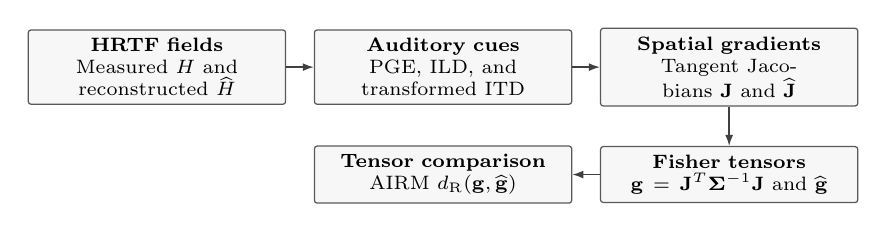
\begin{tikzpicture}[
        node distance=3.5mm,
        stage/.style={
            draw=black!65,
            fill=black!3,
            rounded corners=1pt,
            line width=0.45pt,
            align=center,
            inner xsep=2.5pt,
            inner ysep=3pt,
            font=\scriptsize,
            text width=0.255\columnwidth
        },
        flow/.style={
            -{Latex[length=1.4mm,width=1mm]},
            line width=0.5pt,
            draw=black!75
        }
    ]
        \node[stage] (hrtf) {\textbf{HRTF fields}\\Measured $H$ and reconstructed $\widehat H$};
        \node[stage, right=of hrtf] (cues) {\textbf{Auditory cues}\\PGE, ILD, and transformed ITD};
        \node[stage, right=of cues] (gradients) {\textbf{Spatial gradients}\\Tangent Jacobians $\mathbf J$ and $\widehat{\mathbf J}$};
        \node[stage, below=5mm of gradients] (tensors) {\textbf{Fisher tensors}\\$\mathbf g=\mathbf J^T\boldsymbol\Sigma^{-1}\mathbf J$ and $\widehat{\mathbf g}$};
        \node[stage, left=of tensors] (comparison) {\textbf{Tensor comparison}\\AIRM $d_{\mathrm R}(\mathbf g,\widehat{\mathbf g})$};

        \draw[flow] (hrtf) -- (cues);
        \draw[flow] (cues) -- (gradients);
        \draw[flow] (gradients) -- (tensors);
        \draw[flow] (tensors) -- (comparison);
    \end{tikzpicture}
    \caption{Overview of the proposed evaluation. Measured and reconstructed HRTF fields are transformed into auditory cue fields, differentiated spatially, and compared through their Fisher tensors.}
    \label{fig:evaluation_pipeline}
\end{figure}

\section{Cue Feature Extraction}
Let the source direction be represented by a unit Cartesian vector
\[
\mathbf{r}=[r_x,r_y,r_z]^T\in\mathbb{S}^{2}.
\]
For ear \(c\in\{L,R\}\), let \(A_c(f_k,\mathbf{r})\) and \(\widehat{A}_c(f_k,\mathbf{r})\) denote the target and reconstructed HRTF magnitudes at frequency bin \(f_k\), \(k\in\{1,\ldots,F\}\). Let \(D_c(f_k,\mathbf{r})\) and \(\widehat{D}_c(f_k,\mathbf{r})\) denote their corresponding directional transfer function (DTF) magnitudes after applying the same common-transfer-function (CTF) removal convention. DTF cues are used for the Fisher analysis; raw HRTF magnitudes are retained for signal-domain error metrics.

Three cue functions define the Fisher analysis. They are extracted at measured directions and represented by smooth spherical-harmonic fields, whose spatial derivatives define the tensor.

\subsection{Positive Spectral-Gradient Features (PGE)}
Positive spectral-gradient features follow the sagittal-plane cue convention of Baumgartner et al. \cite{Baumgartner2014} as implemented in the Auditory Modeling Toolbox (AMT) function \path{barumerli2023_featureextraction}. DTF magnitudes are interpolated onto 27 centre frequencies spaced on the equivalent rectangular bandwidth (ERB) rate scale between 0.7 and 18 kHz, converted to dB, and differenced across an approximately one-ERB tonotopic interval. For ear \(c\in\{L,R\}\),
\begin{equation}
S_c[b,\mathbf{r}]
=\max\!\left(m_c[b+d,\mathbf{r}]-m_c[b,\mathbf{r}],0\right),
\end{equation}
where \(m_c[b,\mathbf r]=20\log_{10}(D_c(f_b,\mathbf r)+\varepsilon_A)\), \(b=1,\ldots,B-d\), and \(d\) is selected from the ERB bandwidth model to approximate a one-ERB comparison. The retained positive differences form the monaural spectral cue vector used by the Fisher analysis.
\subsection{Interaural Level Difference (ILD)}
The broadband ILD is defined as the log-ratio of average spectral power across the two ears:
\begin{equation}
\operatorname{ILD}(\mathbf{r})
= 10\log_{10}\!\left(
\frac{\frac{1}{F}\sum_{k=1}^{F} D_L(f_k,\mathbf{r})^2 + \varepsilon_P}
     {\frac{1}{F}\sum_{k=1}^{F} D_R(f_k,\mathbf{r})^2 + \varepsilon_P}
\right).
\end{equation}
Here \(\varepsilon_P>0\) is the power-domain numerical floor used for both target and reconstructed cues.

\subsection{Interaural Time Difference (ITD)}

Let \(a_L(t,\mathbf{r})\) and \(a_R(t,\mathbf{r})\) denote the left- and right-ear head-related impulse responses (HRIRs) at direction \(\mathbf{r}\). For HRTF sets represented as HRIRs, or as complex responses from which HRIRs are obtained by inverse transformation, the broadband ITD field is estimated from the binaural impulse responses:
\begin{equation}
\tau_{\mathrm{ext}}(\mathbf{r})
=
\mathcal{E}_{\mathrm{ITD}}
\!\left[
 a_L(t,\mathbf{r}),a_R(t,\mathbf{r})
\right],
\end{equation}
where \(\mathcal{E}_{\mathrm{ITD}}\) is the Barumerli feature extractor's broadband envelope-correlation estimator, implemented as AMT \path{itdestimator} with the \path{MaxIACCe} convention. For the reported methods, reference and reconstructed HRTFs define separate delay fields,
\begin{equation}
\tau(\mathbf{r})=\tau_{\mathrm{ext}}(\mathbf{r}),
\qquad
\hat{\tau}(\mathbf{r})=\hat{\tau}_{\mathrm{ext}}(\mathbf{r}),
\end{equation}
so that timing errors contribute to the Fisher-tensor comparison.

\noindent The delay is mapped onto the transformed ITD scale used by the observer model \cite{Reijniers2014,Barumerli2023}:
\begin{equation}
\begin{aligned}
T(\tau)=\frac{\operatorname{sgn}(\tau)}{0.095}
\Bigl[&\ln\!\left(32.5\times10^{-6}+0.095|\tau|\right)\\
&-\ln\!\left(32.5\times10^{-6}\right)\Bigr].
\end{aligned}
\end{equation}
This is the Reijniers et al. variance-stabilising transformation for
heteroscedastic ITD discrimination: empirical broadband ITD JNDs increase
approximately linearly with \(|\tau|\), and \(T(\tau)\) is the corresponding
accumulated-JND coordinate. A constant Gaussian noise term on this transformed
coordinate therefore represents constant uncertainty in ITD JND units, not
constant uncertainty in seconds.
The ITD cue used in the spatial cue vector is therefore
\begin{equation}
\operatorname{ITD}(\mathbf{r}) = T\!\left(\tau(\mathbf{r})\right),
\qquad
\widehat{\operatorname{ITD}}(\mathbf{r}) = T\!\left(\hat{\tau}(\mathbf{r})\right).
\end{equation}

\section{Continuous Spatial Gradients and Tangent Projection}
Let the monaural spectral feature vector collect the \(B-d\) PGE values for both ears,
\[
\mathbf{s}(\mathbf{r})\in\mathbb{R}^{N_S},
\qquad N_S=2(B-d).
\]
The full spatial cue vector is
\[
\mathbf{q}(\mathbf{r})
=
\bigl[\mathbf{s}(\mathbf{r})^T,\,\operatorname{ILD}(\mathbf{r}),\,\operatorname{ITD}(\mathbf{r})\bigr]^T
\in\mathbb{R}^{M},
\qquad M=N_S+2.
\]
For a reconstructed HRTF field, the same feature extraction gives
\(\widehat{\mathbf{q}}(\mathbf{r})\) on the same spatial grid.

\subsection{Spherical Harmonic Representation}
Each scalar cue component is represented on the sphere using a truncated real spherical-harmonic (SH) basis of maximum degree \(N_{\max}\). Let
\[
\mathbf{Y}(\mathbf{r}) \in \mathbb{R}^{C}, \qquad C=(N_{\max}+1)^2,
\]
be the vector of basis functions evaluated at \(\mathbf{r}\). Cue samples at fitting directions \(\{\mathbf{r}_n\}_{n=1}^{N_{\mathrm{fit}}}\) are collected in
\[
\mathbf{Q}
=
[\mathbf{q}(\mathbf{r}_1),\ldots,\mathbf{q}(\mathbf{r}_{N_{\mathrm{fit}}})]^T
\in\mathbb{R}^{N_{\mathrm{fit}}\times M},
\]
and the SH design matrix is defined as
\[
\mathbf{Y}_{\mathrm{fit}}
=
[\mathbf{Y}(\mathbf{r}_1),\ldots,\mathbf{Y}(\mathbf{r}_{N_{\mathrm{fit}}})]^T
\in\mathbb{R}^{N_{\mathrm{fit}}\times C}.
\]
The SH coefficient matrix \(\mathbf{B}\in\mathbb{R}^{C\times M}\) is obtained by least squares:
\begin{equation}
\mathbf{B} = \mathbf{Y}_{\mathrm{fit}}^{\dagger}\mathbf{Q},
\end{equation}
where \(\mathbf{Y}_{\mathrm{fit}}^{\dagger}\) denotes the Moore--Penrose pseudoinverse. When \(\mathbf{Y}_{\mathrm{fit}}\) has full column rank,
\begin{equation}
\mathbf{Y}_{\mathrm{fit}}^{\dagger}
=
\left(\mathbf{Y}_{\mathrm{fit}}^T\mathbf{Y}_{\mathrm{fit}}\right)^{-1}
\mathbf{Y}_{\mathrm{fit}}^T.
\end{equation}
The smooth cue field is
\begin{equation}
\widetilde{\mathbf{q}}(\mathbf{r}) = \mathbf{B}^{T}\mathbf{Y}(\mathbf{r}).
\end{equation}
For the reconstructed HRTF field, define
\[
\widehat{\mathbf{Q}}
=
[\widehat{\mathbf{q}}(\mathbf{r}_1),\ldots,\widehat{\mathbf{q}}(\mathbf{r}_{N_{\mathrm{fit}}})]^T .
\]
It is fitted with the same \(N_{\max}\), basis convention, and fitting grid:
\begin{equation}
\widehat{\mathbf{B}} = \mathbf{Y}_{\mathrm{fit}}^{\dagger}\widehat{\mathbf{Q}},
\qquad
\widehat{\widetilde{\mathbf{q}}}(\mathbf{r})
=
\widehat{\mathbf{B}}^T\mathbf{Y}(\mathbf{r}).
\end{equation}
The main evaluation uses \(N_{\max}=6\) for both fields. Using the same SH order makes their gradients comparable at the same spatial resolution. This cue-field fit is separate from the SH interpolation used by some reconstruction methods.

\subsection{Continuous Spatial Derivatives}

The SH representation provides a smooth approximation to each cue field, allowing spatial derivatives to be evaluated at arbitrary directions. Let
\[
\mathbf{J}_{\mathbf{Y}}(\mathbf{r}) =
\nabla_{\mathbf{r}}\mathbf{Y}(\mathbf{r})
\in \mathbb{R}^{C\times 3}.
\]
The Cartesian cue Jacobian is then
\begin{equation}
\mathbf{J}_{\mathrm{Cart}}(\mathbf{r})
=
\nabla_{\mathbf{r}}\widetilde{\mathbf{q}}(\mathbf{r})
=
\mathbf{B}^{T}\mathbf{J}_{\mathbf{Y}}(\mathbf{r}).
\end{equation}

\subsection{Local Tangent Plane Projection}
Because source direction lies on the unit sphere, only tangential variations are relevant for local discriminability. The unit normal at \(\mathbf{r}\) is \(\mathbf{r}\) itself. A local orthonormal tangent basis \(\mathbf{V}(\mathbf{r})=[\mathbf{u}_1,\mathbf{u}_2]\in\mathbb{R}^{3\times2}\) is defined by selecting an auxiliary vector
\[
\mathbf{h}_{\mathrm{aux}} =
\begin{cases}
 [0,1,0]^T, & \text{if } |r_z| > 0.9,\\
 [0,0,1]^T, & \text{otherwise},
\end{cases}
\]
and then setting
\begin{equation}
\mathbf{u}_1 = \frac{\mathbf{h}_{\mathrm{aux}}\times \mathbf{r}}{\|\mathbf{h}_{\mathrm{aux}}\times \mathbf{r}\|_2},
\qquad
\mathbf{u}_2 = \mathbf{r} \times \mathbf{u}_1.
\end{equation}
The same basis is used for target and reconstruction at each direction. Since \(\mathbf{r}\) is unit length, its tangent coordinates describe infinitesimal angular displacement in radians. The tangent Jacobian is
\begin{equation}
\mathbf{J}_{\mathrm{tan}}(\mathbf{r}) =
\mathbf{J}_{\mathrm{Cart}}(\mathbf{r})\,\mathbf{V}(\mathbf{r})
\in \mathbb{R}^{M\times2}.
\end{equation}

\section{Construction of the Fisher--Rao Metric Tensor}
For the Fisher analysis, cue observations are modelled locally as Gaussian with mean \(\widetilde{\mathbf{q}}(\mathbf{r})\) and direction-independent covariance \(\boldsymbol{\Sigma}\). Following the independent-feature covariance used by Barumerli et al. \cite{Barumerli2023}, cue-family noise is represented by the block-diagonal matrix
\begin{equation}
\boldsymbol{\Sigma} = 
\begin{bmatrix}
\sigma_{\mathrm{mon}}^2 \mathbf{I}_{N_S} & \mathbf{0} & \mathbf{0} \\
\mathbf{0}^T & \sigma_{\mathrm{ILD}}^2 & 0 \\
\mathbf{0}^T & 0 & \sigma_{\mathrm{ITD}}^2
\end{bmatrix},
\end{equation}
where \(\mathbf{I}_{N_S}\) is the \(N_S\times N_S\) identity matrix. The off-diagonal entries of \(\mathbf{g}(\mathbf{r})\) are the precision-weighted inner products between tangent cue gradients.

The standard deviations set the relative cue weights. The analysis uses \(\sigma_{\mathrm{mon}}=1.25\,\mathrm{dB}\), \(\sigma_{\mathrm{ILD}}=1\,\mathrm{dB}\), and \(\sigma_{\mathrm{ITD}}=0.569\) on the transformed \(T(\tau)\) scale. The ITD value is the Reijniers et al. discrimination-derived standard deviation on the transformed JND coordinate \cite{Reijniers2014}. The PGE and ILD values are the medians of the listener-specific gradient-profile fits reported by Barumerli et al. \cite{Barumerli2023}. They are effective observer-model weights calibrated using separate localisation responses, rather than direct physiological measurements of internal noise, and are not fitted to the behavioural thresholds discussed below. The Bayesian evaluation additionally includes the observer prior, decision rule, and response stage.

For the diagonal Gaussian covariance defined by these standard deviations, the Fisher information matrix on the two-dimensional tangent space is
\begin{equation}
\mathbf{g}(\mathbf{r}) =
\mathbf{J}_{\mathrm{tan}}(\mathbf{r})^T\,
\boldsymbol{\Sigma}^{-1}\,
\mathbf{J}_{\mathrm{tan}}(\mathbf{r})
\in \mathbb{R}^{2\times2}.
\end{equation}
Let \(\mathbf{j}_{u}(\mathbf{r})=\nabla_{\mathrm{tan}}u(\mathbf{r})\in\mathbb{R}^{2}\) denote the tangent gradient of a scalar cue \(u\). The FIM can be written explicitly as
\begin{equation}
\begin{aligned}
\mathbf{g}(\mathbf{r})={}&
\frac{1}{\sigma_{\mathrm{mon}}^2}
\sum_{c\in\{L,R\}}\sum_{b=1}^{B-d}
\mathbf{j}_{S_c[b]}\mathbf{j}_{S_c[b]}^T\\
&+\frac{1}{\sigma_{\mathrm{ILD}}^2}
\mathbf{j}_{\mathrm{ILD}}\mathbf{j}_{\mathrm{ILD}}^T
+\frac{1}{\sigma_{\mathrm{ITD}}^2}
\mathbf{j}_{\mathrm{ITD}}\mathbf{j}_{\mathrm{ITD}}^T,
\end{aligned}
\end{equation}
where every cue gradient on the right-hand side is evaluated at
\(\mathbf{r}\).
Thus, \(\mathbf{g}\) is positive semidefinite and is positive definite only where the weighted cue gradients span both tangent directions. Strict positive definiteness for tensor comparison is supplied by the regularisation defined below.

Figures~\ref{fig:sonicom_kent} and~\ref{fig:kent_map_scatter} place the two observer summaries side by side. The CRB ellipses describe local cue sensitivity before the prior, decision, and response stages. The Barumerli ellipses describe the covariance of the complete simulated response and include its isotropic sensorimotor-scatter component.

\begin{figure*}[t]
    \centering
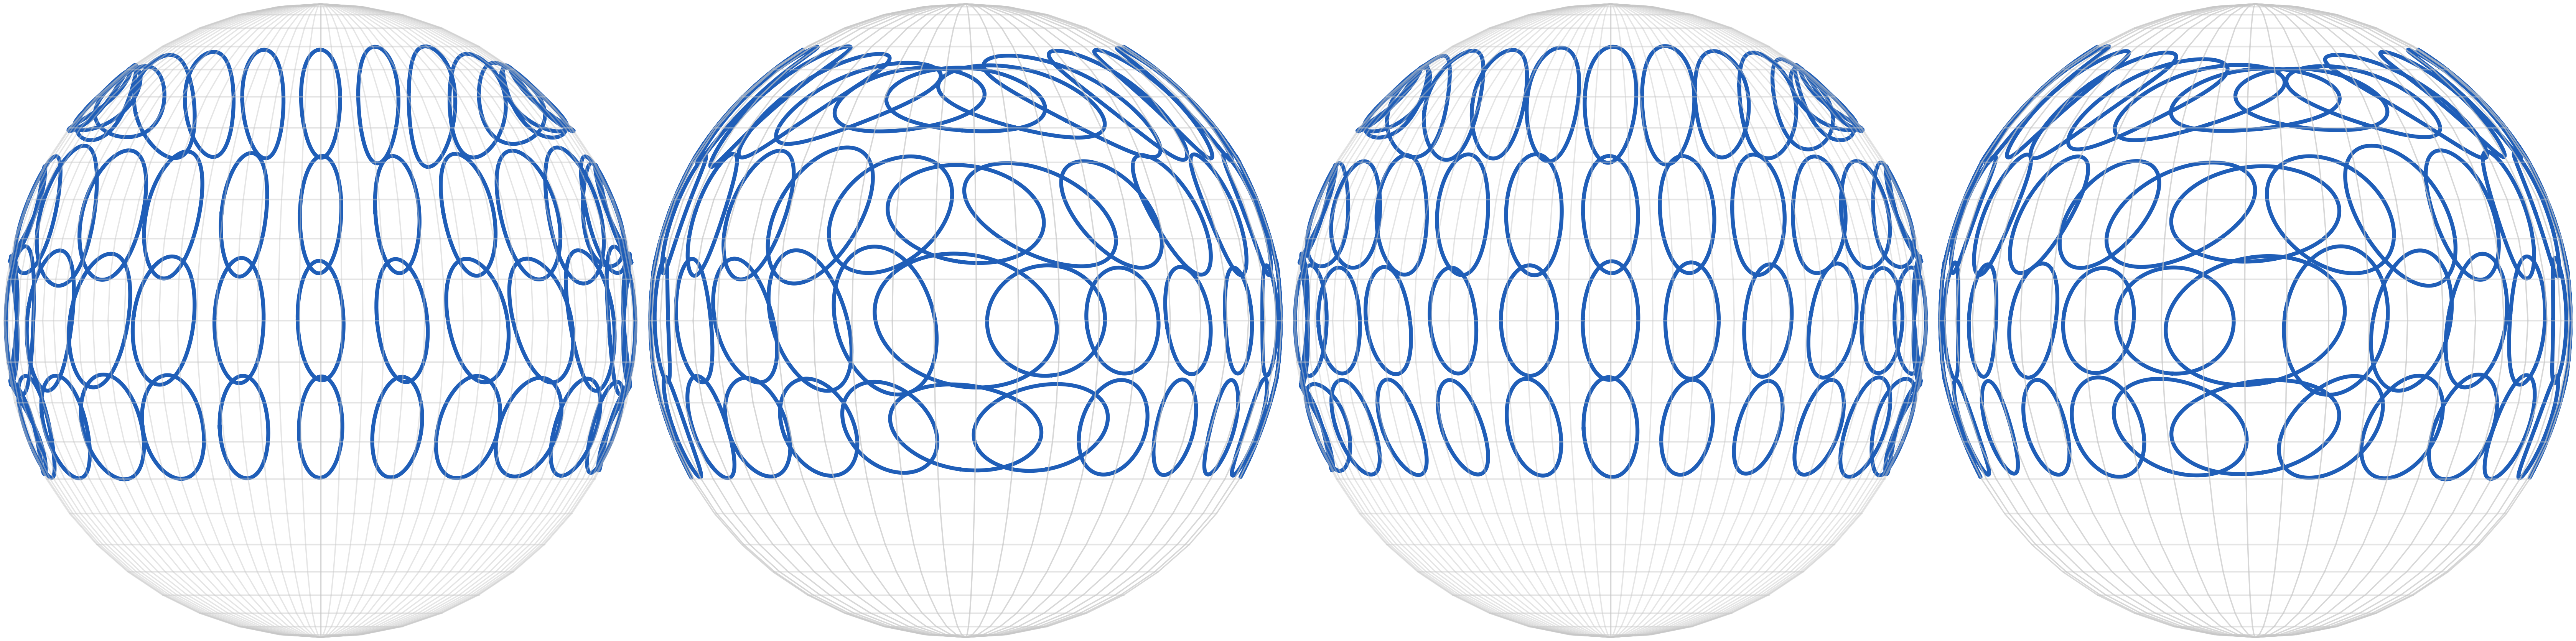
\includegraphics[width=0.92\textwidth]{figures/evaluation/median_crb_ellipses.png}
    \caption[SONICOM Fisher discriminability ellipses from the Cram\'er--Rao bound]{Local auditory discrimination ellipses derived from the Cram\'er--Rao bound. Ellipses show the 95\% contour of a bivariate Gaussian with covariance equal to the CRB, scaled by \(\sqrt{\chi^2_{2,0.95}}\). Views correspond to azimuths of \(0^\circ\), \(90^\circ\), \(180^\circ\), and \(270^\circ\). Results are based on the median Fisher tensor of the 41-subject SONICOM evaluation cohort.}
    \label{fig:sonicom_kent}
\end{figure*}

\begin{figure*}[t]
    \centering
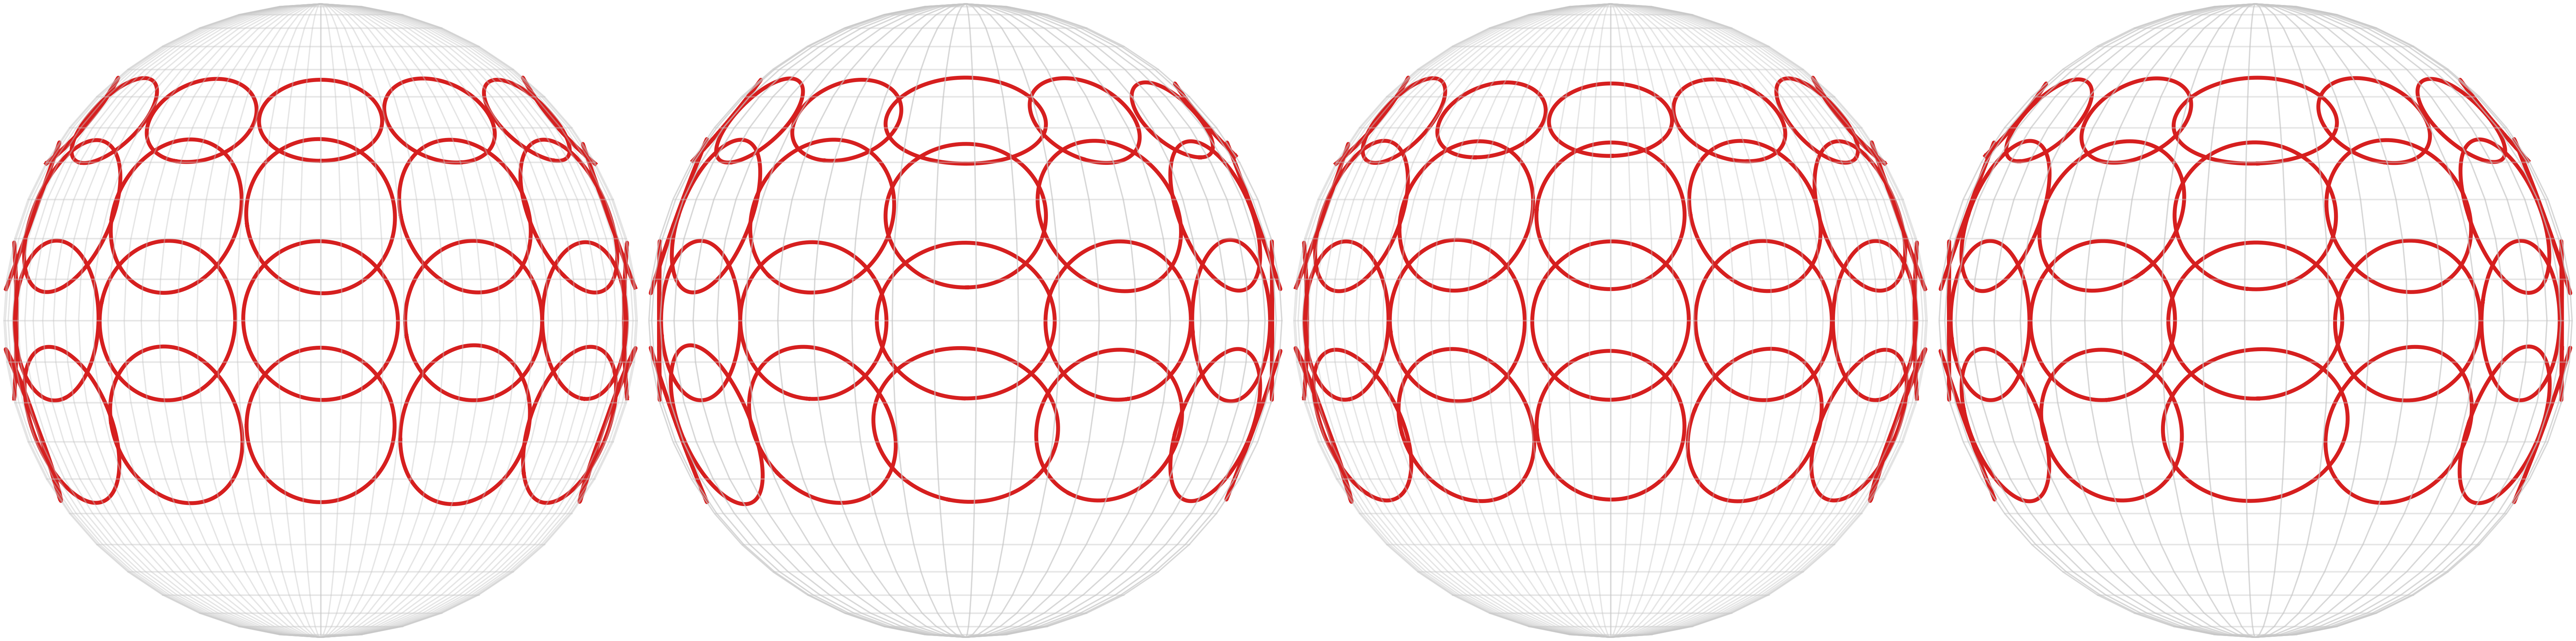
\includegraphics[width=0.92\textwidth]{figures/evaluation/median_barumerli_map_response_covariance.png}
    \caption[Predicted pointing-error covariance from the Barumerli MAP estimator]{Predicted pointing error from a converged Monte Carlo simulation of the maximum a posteriori estimator of Barumerli et al. \cite{Barumerli2023}. Ellipses represent local response covariance matrices, scaled to one standard deviation along each principal axis. Views correspond to azimuths of \(0^\circ\), \(90^\circ\), \(180^\circ\), and \(270^\circ\). Results are based on the median covariance of the 41-subject SONICOM evaluation cohort.}
    \label{fig:kent_map_scatter}
\end{figure*}

\section{AIRM Tensor Discrepancy}
The target and reconstructed Fisher tensors are compared using the affine-invariant Riemannian metric (AIRM) on symmetric positive-definite matrices. Since empirical Fisher tensors may be singular where the weighted cue gradients do not span both tangent directions, both fields are symmetrised and regularised by the same diagonal term,
\begin{equation}
\mathbf{g}_{\eta}(\mathbf{r})=\mathbf{g}(\mathbf{r})+\eta\mathbf{I}_2,
\qquad
\widehat{\mathbf{g}}_{\eta}(\mathbf{r})
=
\widehat{\mathbf{g}}(\mathbf{r})+\eta\mathbf{I}_2,
\end{equation}
with \(\eta=10^{-6}\). The pointwise tensor discrepancy is
\begin{equation}
 d_{\mathrm{AIRM}}(\mathbf{g}_{\eta},\widehat{\mathbf{g}}_{\eta})
 =
 \left\|\log\!\left(
 \mathbf{g}_{\eta}^{-1/2}
 \widehat{\mathbf{g}}_{\eta}
 \mathbf{g}_{\eta}^{-1/2}
 \right)\right\|_F .
\end{equation}
For a \(2\times2\) tensor pair this is evaluated from the positive generalised eigenvalues \(\lambda_1,\lambda_2\) of \((\widehat{\mathbf{g}}_{\eta},\mathbf{g}_{\eta})\):
\begin{equation}
 d_{\mathrm{AIRM}}
 =
 \sqrt{\log^2(\lambda_1)+\log^2(\lambda_2)}.
\end{equation}
Numerically, the same result is obtained by Cholesky congruence: if \(\mathbf{g}_{\eta}=\mathbf L\mathbf L^T\), the eigenvalues are computed from the symmetrised matrix \(\mathbf L^{-1}\widehat{\mathbf g}_{\eta}\mathbf L^{-T}\), with eigenvalues floored at \(10^{-12}\) before taking logarithms. The mean AIRM discrepancy over the evaluation grid \(\{\mathbf r_n\}_{n=1}^{N_{\mathrm{eval}}}\) is
\begin{equation}
\mathcal{E}_{\mathrm{AIRM}} =
\frac{1}{N_{\mathrm{eval}}}\sum_{n=1}^{N_{\mathrm{eval}}}
 d_{\mathrm{AIRM}}\bigl(\mathbf g_\eta(\mathbf r_n),
 \widehat{\mathbf g}_\eta(\mathbf r_n)\bigr).
\label{eq:mean_airm}
\end{equation}
\section{Evaluation Metrics}
AIRM measures the distance between reference and reconstructed Fisher tensors. Signal-domain metrics measure physical reconstruction error, and the Bayesian-observer metrics summarise simulated localisation responses.

\subsection{Log-Spectral Distortion (LSD)}
Using the HRTF-magnitude notation defined above, the binaural log-spectral distortion is
\begin{equation}
\begin{aligned}
\operatorname{LSD}
={}&\frac{1}{N_{\mathrm{eval}}}
\sum_{n=1}^{N_{\mathrm{eval}}}\Biggl[
\frac{1}{2W}\sum_{c\in\{L,R\}}\sum_{w=1}^{W}\\
&\left(
20\log_{10}
\frac{A_c(f_w,\mathbf{r}_n)+\varepsilon_A}
{\widehat{A}_c(f_w,\mathbf{r}_n)+\varepsilon_A}
\right)^2\Biggr]^{1/2}.
\end{aligned}
\end{equation}
LSD serves as the principal signal-domain metric because it directly measures spectral magnitude agreement. For the HRIR/SOFA reconstructions evaluated here, LSD is computed over the common LAP/SAM band from 20 Hz to 20 kHz, except for FSP-AE, whose configured output extends to 16 kHz. Both reference and reconstructed spectra are restricted to this band for the FSP-AE comparison.

\subsection{Interaural Level Difference Error}
ILD error measures binaural level reconstruction. Define the frequency-averaged HRTF ILD
\begin{equation}
\operatorname{ILD}_{\mathrm{HRTF}}(\mathbf{r})
=
\frac{1}{F}\sum_{k=1}^{F}
20\log_{10}\!\left(
\frac{A_L(f_k,\mathbf{r})+\varepsilon_A}
     {A_R(f_k,\mathbf{r})+\varepsilon_A}
\right),
\end{equation}
with reconstruction error
\begin{equation}
\mathcal{E}_{\mathrm{ILD}}
=
\frac{1}{N_{\mathrm{eval}}}\sum_{n=1}^{N_{\mathrm{eval}}}
\left|
\operatorname{ILD}_{\mathrm{HRTF}}(\mathbf{r}_n)
-\widehat{\operatorname{ILD}}_{\mathrm{HRTF}}(\mathbf{r}_n)
\right|.
\end{equation}
This signal-domain quantity differs from the broadband DTF power-ratio ILD cue used in the Fisher tensor. One measures error in the binaural level field; the other contributes its spatial derivatives to the Fisher matrix.

\subsection{Fisher-Tensor AIRM Discrepancy}
The primary tensor metric is the mean AIRM discrepancy in \eqref{eq:mean_airm}. It compares the scale, anisotropy, and orientation of the Fisher tensors formed from the spatial cue gradients.

The scalar AIRM score is supplemented by tensor summaries. Let \(\mu_1(\mathbf{r})\geq\mu_2(\mathbf{r})>0\) be the eigenvalues of \(\mathbf{g}_{\eta}(\mathbf{r})\), and let \(\mathbf{v}_1(\mathbf{r})\) be its principal information direction. The reported summaries are
\begin{align}
\mathcal{E}_{\mathrm{det}} &=
\frac{1}{N_{\mathrm{eval}}}\sum_n
\left|\log\frac{\det\widehat{\mathbf{g}}_{\eta}(\mathbf{r}_n)}
{\det\mathbf{g}_{\eta}(\mathbf{r}_n)}\right|, \\
\mathcal{E}_{\mathrm{anis}} &=
\frac{1}{N_{\mathrm{eval}}}\sum_n
\left|\log\frac{\hat{\mu}_1(\mathbf{r}_n)/\hat{\mu}_2(\mathbf{r}_n)}
{\mu_1(\mathbf{r}_n)/\mu_2(\mathbf{r}_n)}\right|, \\
\mathcal{E}_{\mathrm{orient}} &=
\frac{1}{|\mathcal{R}_{\mathrm{aniso}}|}
\sum_{\mathbf{r}_n\in\mathcal{R}_{\mathrm{aniso}}}
\arccos\left(
\left|\widehat{\mathbf{v}}_1(\mathbf{r}_n)^T\mathbf{v}_1(\mathbf{r}_n)\right|
\right),
\end{align}
where \(\mathcal{R}_{\mathrm{aniso}}\) contains the directions for which both tensors satisfy \(\mu_1/\mu_2 \geq 1.10\). The orientation error is reported in degrees. The determinant, anisotropy, and orientation summaries describe complementary aspects of the changes measured jointly by AIRM.

\subsection{Bayesian Localisation Metrics}
A Bayesian localisation model supplies lateral RMS error, local polar RMS error, and quadrant error \cite{Middlebrooks1999,Barumerli2023}. Let \(\ell_i,\varphi_i\) denote the lateral and polar target angles and \(\widetilde{\ell}_i,\widetilde{\varphi}_i\) their simulated responses for \(N_{\mathrm{trial}}\) responses, where \(N_{\mathrm{trial}}\) includes the simulated repetitions over the dense target-direction set. For the polar-error target set \(\mathcal{P}\), define local polar responses by
\[
\mathcal{A}=
\left\{i\in\mathcal{P}:
\left|\operatorname{wrap}(\widetilde{\varphi}_i-\varphi_i)\right|<90^\circ
\right\}.
\]
The reported metrics are
\begin{equation}
\operatorname{Lateral~RMS}=
\sqrt{\frac{1}{N_{\mathrm{trial}}}
\sum_{i=1}^{N_{\mathrm{trial}}}
(\widetilde{\ell}_i-\ell_i)^2},
\end{equation}
\begin{equation}
\operatorname{Local~Polar~RMS}=
\sqrt{\frac{1}{|\mathcal{A}|}
\sum_{i\in\mathcal{A}}
\operatorname{wrap}(\widetilde{\varphi}_i-\varphi_i)^2},
\end{equation}
\begin{equation}
\operatorname{Quadrant~Error}
=
\left(1-\frac{|\mathcal{A}|}{|\mathcal{P}|}\right)\times100.
\end{equation}
The implementation uses AMT \path{barumerli2023} with DTF feature extraction, maximum a posteriori estimation, and \(R=300\) simulated repetitions per target direction. Its parameters are \(\sigma_{\mathrm{ITD}}=0.569\), \(\sigma_{\mathrm{ILD}}=1\), \(\sigma_{\mathrm{spectral}}=4\), \(\sigma_{\mathrm{prior}}=11.5\), and \(\sigma_{\mathrm{motor}}=14\). The DTF representation and spectral-noise value follow the public HRTFformer localisation evaluation \cite{Hu2026HRTFformer}; the other parameters follow the AMT 1.6 \path{barumerli2023} defaults. The DTF spectral-noise parameter is distinct from the PGE weight \(\sigma_{\mathrm{mon}}=1.25\) used to construct the Fisher tensors. The resulting metrics summarise simulated pointing after application of the complete observer model.

\section{Evaluation Procedure}
\subsection{Data and Spatial Conditions}\label{sec:data}
The evaluation uses the 48-kHz \path{FreeFieldCompMinPhase} version of the SONICOM HRTF dataset \cite{Engel2023} with a 162/41 train--test split. Here, \emph{MinPhase} denotes the minimum-phase inverse filter used for free-field compensation, not a minimum-phase reconstruction of each HRTF. The retained-direction counts and sparse masks follow the SONICOM upsampling protocol used by Hu et al. for HRTFformer, within the broader LAP upsampling benchmark context \cite{Hu2026HRTFformer,Hogg2025LAPUpsampling}. RANF, FSP-AE, and the interpolation methods use the same 41 held-out subjects and sparse masks. A 512-point FFT gives 256 non-DC bins per ear, or 512 binaural magnitude values per direction, on the dense grid of 793 directions.

Four sparse-to-dense conditions are evaluated: \(100\rightarrow793\), \(19\rightarrow793\), \(5\rightarrow793\), and \(3\rightarrow793\). The same retained directions are used for every method and subject within each condition (Fig.~\ref{fig:sampling_scheme}).

\begin{figure}[t]
    \centering
    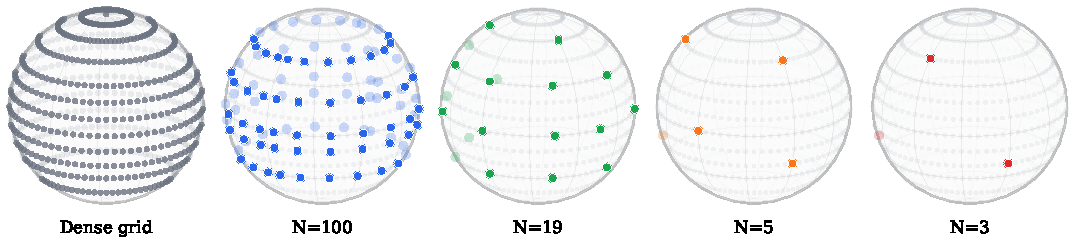
\includegraphics[width=\columnwidth]{figures/evaluation/sampling_scheme_overview.pdf}
    \caption[Dense and sparse SONICOM sampling schemes]{Dense SONICOM evaluation grid and retained sparse sampling schemes used for the four upsampling conditions. Grey points denote the dense 793-direction target grid; coloured points denote retained directions.}
    \label{fig:sampling_scheme}
\end{figure}

All Fisher-tensor fitting and AIRM comparison are performed on the unique physical grid. Duplicate coordinate entries introduced by an implementation layout receive no additional weight.

\subsection{Compared Reconstruction Methods}
The evaluation requires a reconstructed HRTF field on the common evaluation grid. The SUpDEq configurations follow the directional equalisation approach of P\"orschmann et al. \cite{Poerschmann2019SUpDEq}. The reported comparison includes:
\begin{enumerate}
    \item \textbf{SUpDEq-SH:} SUpDEq preprocessing followed by SH interpolation.
    \item \textbf{SUpDEq-MCA:} the published Magnitude-Corrected and Time-Aligned configuration, which uses the same SH interpolation stage and then applies magnitude correction.
    \item \textbf{Natural- and barycentric-MCA variants:} SUpDEq variants with magnitude-correction boosts limited to \(6\,\mathrm{dB}\), using natural-neighbour and barycentric interpolation, respectively.
    \item \textbf{RANF:} a retrieval-augmented neural field that predicts magnitude and ITD and reconstructs HRIRs using a minimum-phase representation with ITD compensation \cite{Masuyama2025RANF,Masuyama2025ICASSPRANF}.
    \item \textbf{FSP-AE:} a neural network conditioned on source position and frequency that predicts HRTF magnitude and ITD before HRIR reconstruction \cite{Ito2025FSPAE}.
\end{enumerate}
The natural-neighbour variant uses Voronoi-weighted interpolation as implemented by the SFS/SUpDEq routines. SUpDEq-Bary-MCA is undefined at three retained directions because they cannot form the required closed spherical hull; this condition is marked not applicable.

For SUpDEq calls using SH interpolation, the reconstruction order is capped at \(\min(6,\lfloor\sqrt{N_{\mathrm{ret}}}-1\rfloor)\), where \(N_{\mathrm{ret}}\) is the number of retained directions. This avoids fitting more SH coefficients than the sparse grid can support. At \(N_{\mathrm{ret}}=3\), the cap therefore gives a zeroth-order SH magnitude field; methods without a direction-dependent delay or correction stage can consequently yield nearly constant cue fields. The Fisher-tensor metric records this behaviour as interpolation failure.

\subsection{Preprocessing and Reconstruction Normalisation}
All methods are converted to a common representation before comparison. Left- and right-ear HRTF magnitudes are aligned on the same frequency bins, with the DC bin removed. Methods operating in the SH domain are inverse-transformed to the full spatial grid; methods outputting HRIRs are converted to magnitudes by a common procedure. Fisher cues are extracted using the Barumerli PGE, ILD, and \path{MaxIACCe} ITD convention. RANF and FSP-AE are evaluated from their full model-generated HRIR/SOFA fields with model-provided ITD. Measured HRIRs are not substituted at the retained nodes.

The same CTF removal is applied to target and reconstruction before DTF feature extraction, leaving the direction-dependent spectral variation used to form the Fisher tensors.

\section{Results}
\subsection{Evaluation Coverage}
The comparison covers 41 subjects, four retention conditions, and six reconstruction methods. SUpDEq-Bary-MCA is not applicable at \(N=3\), leaving 943 subject--method--condition combinations across 23 method--retention conditions. AIRM, LSD, ILD, and Bayesian localisation metrics were obtained for all 943 combinations.

\begin{figure*}[t]
    \centering
    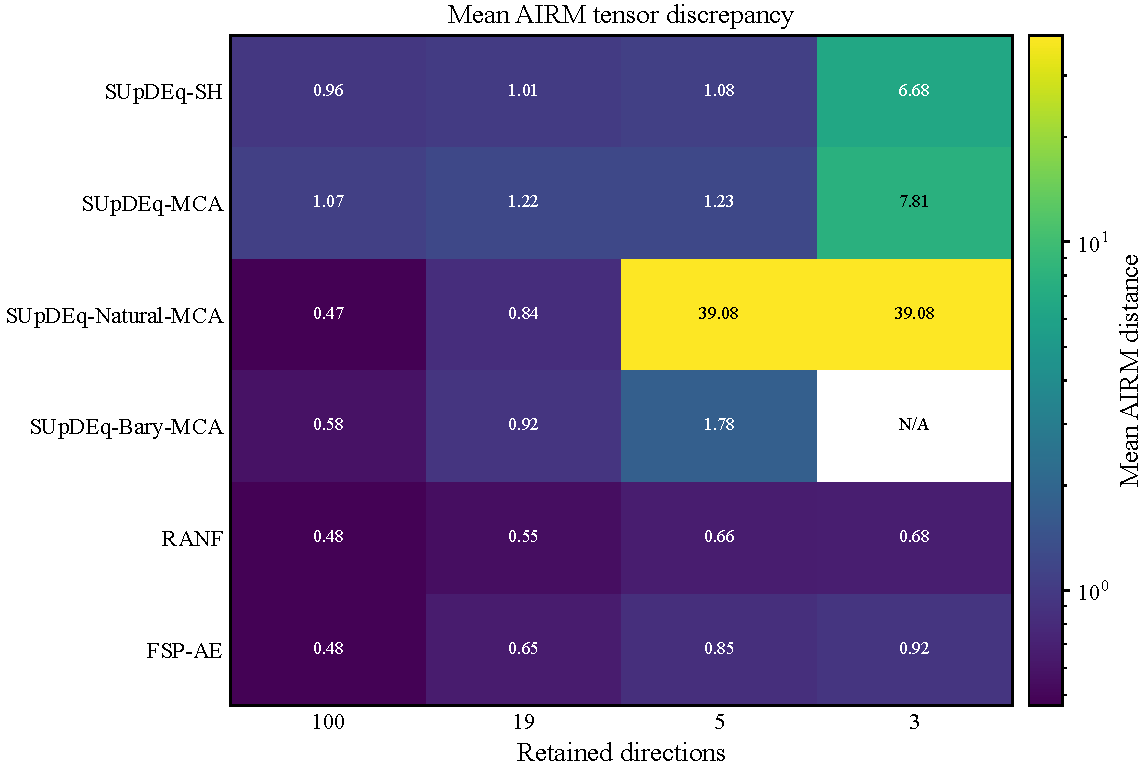
\includegraphics[width=0.70\textwidth]{figures/evaluation/airm_heatmap.pdf}
    \caption[Mean AIRM discrepancy over methods and retention conditions]{Mean Fisher-tensor AIRM discrepancy over the 41-subject cohort. Lower values indicate closer preservation of the dense-reference tensor field; the blank entry is the not-applicable \(N=3\) SUpDEq-Bary-MCA condition.}
    \label{fig:airm_heatmap}
\end{figure*}

\subsection{Fisher-Tensor Results}
Figure~\ref{fig:airm_heatmap} reports cohort-mean AIRM for the six reconstruction methods. RANF gives the lowest mean AIRM at \(N=19\), \(N=5\), and \(N=3\), with FSP-AE second. At \(N=100\), SUpDEq-Natural-MCA is slightly lower (0.47) than RANF and FSP-AE (both 0.48). RANF's mean AIRM increases to 0.68 at \(N=3\). Among the interpolation methods, SUpDEq-Natural-MCA and SUpDEq-Bary-MCA are strongest at \(N=100\) and \(N=19\), but SUpDEq-Natural-MCA produces very large AIRM discrepancies at \(N=5\) and \(N=3\). SUpDEq-Bary-MCA is not applicable at \(N=3\).

AIRM depends on local derivatives and on tensor anisotropy and orientation, so its method ranking can differ from rankings based on LSD or Bayesian-observer summaries.

Sensitivity to the Fisher-field settings was assessed without changing the subjects, masks, reconstructed fields, cue model, or AIRM implementation. Repeating the principal RANF--FSP-AE comparison with cue-field SH orders 4, 6, and 8 preserved the cohort ordering RANF \(<\) FSP-AE at \(N=3\), \(N=5\), and \(N=19\). At \(N=100\), their AIRM values were nearly equal and the small lead changed with SH order, so this condition is not interpreted as a meaningful distinction. Recomputing AIRM with \(\eta=10^{-8}\), \(10^{-6}\), and \(10^{-4}\) did not change the ranking among conditions with finite AIRM values.

Table~\ref{tab:tensor_component_means} reports cohort-mean errors in tensor scale, anisotropy, and principal-axis direction. Orientation error is evaluated only where both reference and reconstructed tensors are sufficiently anisotropic for a principal-axis angle to be meaningful.

\begin{table*}[t]
\centering
\caption{Mean secondary Fisher-tensor component errors over the 41-subject cohort for the principal comparison set. Dashes denote conditions that are not applicable or for which the component summary is undefined under the stated validity criteria.}
\label{tab:tensor_component_means}
\scriptsize
\begin{tabular}{llrrrr}
\toprule
Component & Method & $N=100$ & $N=19$ & $N=5$ & $N=3$ \\
\midrule
Log-det. & SUpDEq-SH & 0.70 & 0.68 & 0.87 & 7.14 \\
Log-det. & SUpDEq-MCA & 0.90 & 0.95 & 0.97 & 8.70 \\
Log-det. & SUpDEq-Natural-MCA & 0.32 & 0.69 & -- & -- \\
Log-det. & SUpDEq-Bary-MCA & 0.37 & 0.67 & 1.31 & -- \\
Log-det. & RANF & 0.34 & 0.39 & 0.47 & 0.50 \\
Log-det. & FSP-AE & 0.36 & 0.57 & 0.81 & 0.91 \\
\addlinespace
Anisotropy & SUpDEq-SH & 0.56 & 0.67 & 0.67 & 5.80 \\
Anisotropy & SUpDEq-MCA & 0.57 & 0.68 & 0.80 & 6.41 \\
Anisotropy & SUpDEq-Natural-MCA & 0.31 & 0.54 & -- & -- \\
Anisotropy & SUpDEq-Bary-MCA & 0.38 & 0.54 & 1.43 & -- \\
Anisotropy & RANF & 0.32 & 0.37 & 0.44 & 0.45 \\
Anisotropy & FSP-AE & 0.32 & 0.43 & 0.54 & 0.59 \\
\addlinespace
Orientation ($^\circ$) & SUpDEq-SH & 18.9 & 20.2 & 16.4 & 13.0 \\
Orientation ($^\circ$) & SUpDEq-MCA & 19.3 & 22.5 & 17.1 & 13.2 \\
Orientation ($^\circ$) & SUpDEq-Natural-MCA & 7.2 & 11.3 & -- & -- \\
Orientation ($^\circ$) & SUpDEq-Bary-MCA & 8.6 & 14.3 & 17.7 & -- \\
Orientation ($^\circ$) & RANF & 6.8 & 8.9 & 10.7 & 10.6 \\
Orientation ($^\circ$) & FSP-AE & 7.2 & 8.6 & 9.6 & 9.6 \\
\bottomrule
\end{tabular}
\end{table*}


\subsection{Signal and Bayesian-Observer Metrics}
Conventional and Bayesian-observer metrics were computed for every completed method--condition--subject row. The Bayesian localisation model produces absolute simulated errors, but the manuscript reports the boxplot summaries relative to the dense self-reference condition for the same subject and observer configuration. These are signed changes in simulated error: positive values indicate greater error than the dense self-reference, while negative values indicate lower simulated error. The self-reference remains non-zero because the observer includes sensory noise, a prior, a decision rule, and response scatter.

RANF has the lowest LSD throughout the evaluated retention conditions. FSP-AE has larger LSD than RANF, but is competitive with the interpolation baselines and remains spectrally stable as sparsity increases. It also avoids the large Fisher-tensor discrepancies observed for several interpolation baselines. Among the interpolation methods, AIRM, LSD, and relative Bayesian-observer summaries do not always select the same reconstruction. The three evaluations measure tensor preservation, spectral reconstruction, and simulated localisation, respectively.

\begin{figure}[!t]
    \centering
    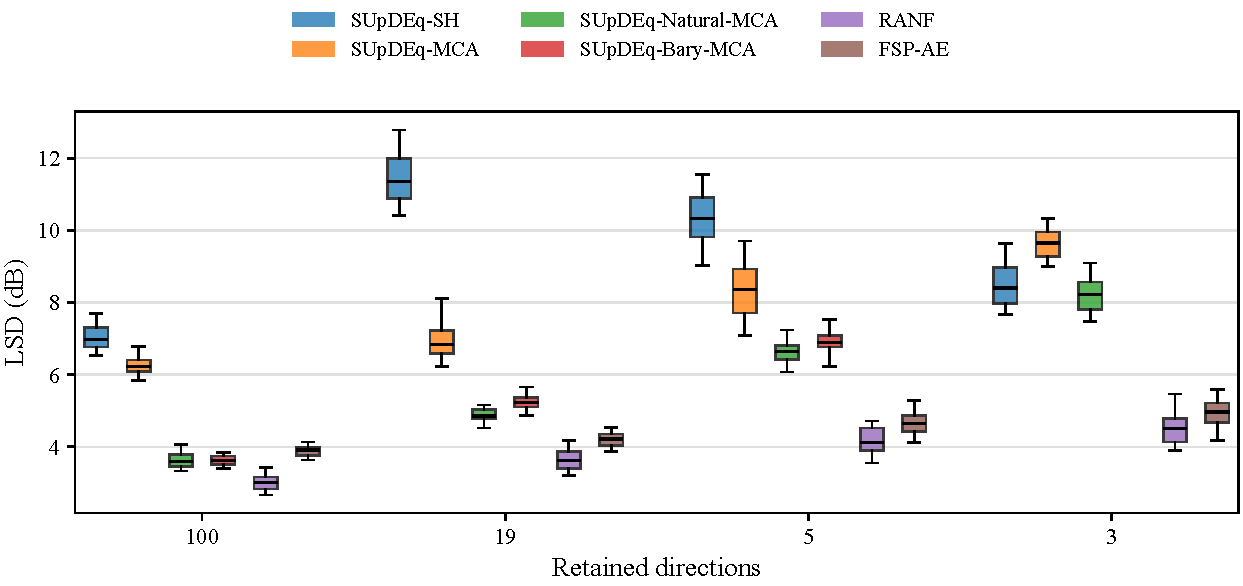
\includegraphics[width=\columnwidth]{figures/evaluation/lsd_subject_boxplot.pdf}
    \caption[Subject-wise LSD distributions]{Subject-wise LSD distributions over the 41 held-out subjects. Boxes show medians and interquartile ranges; whiskers span the 5th--95th percentiles.}
    \label{fig:lsd_subject_boxplot}
\end{figure}

Figure~\ref{fig:bayesian_subject_distributions} reports subject-wise distributions for lateral RMS, local polar RMS, and quadrant error. Lateral RMS measures error in lateral angle, including both bias and response variability. Local polar RMS measures polar error within the correct quadrant; quadrant error counts larger polar confusions.

\begin{figure}[!t]
    \centering
    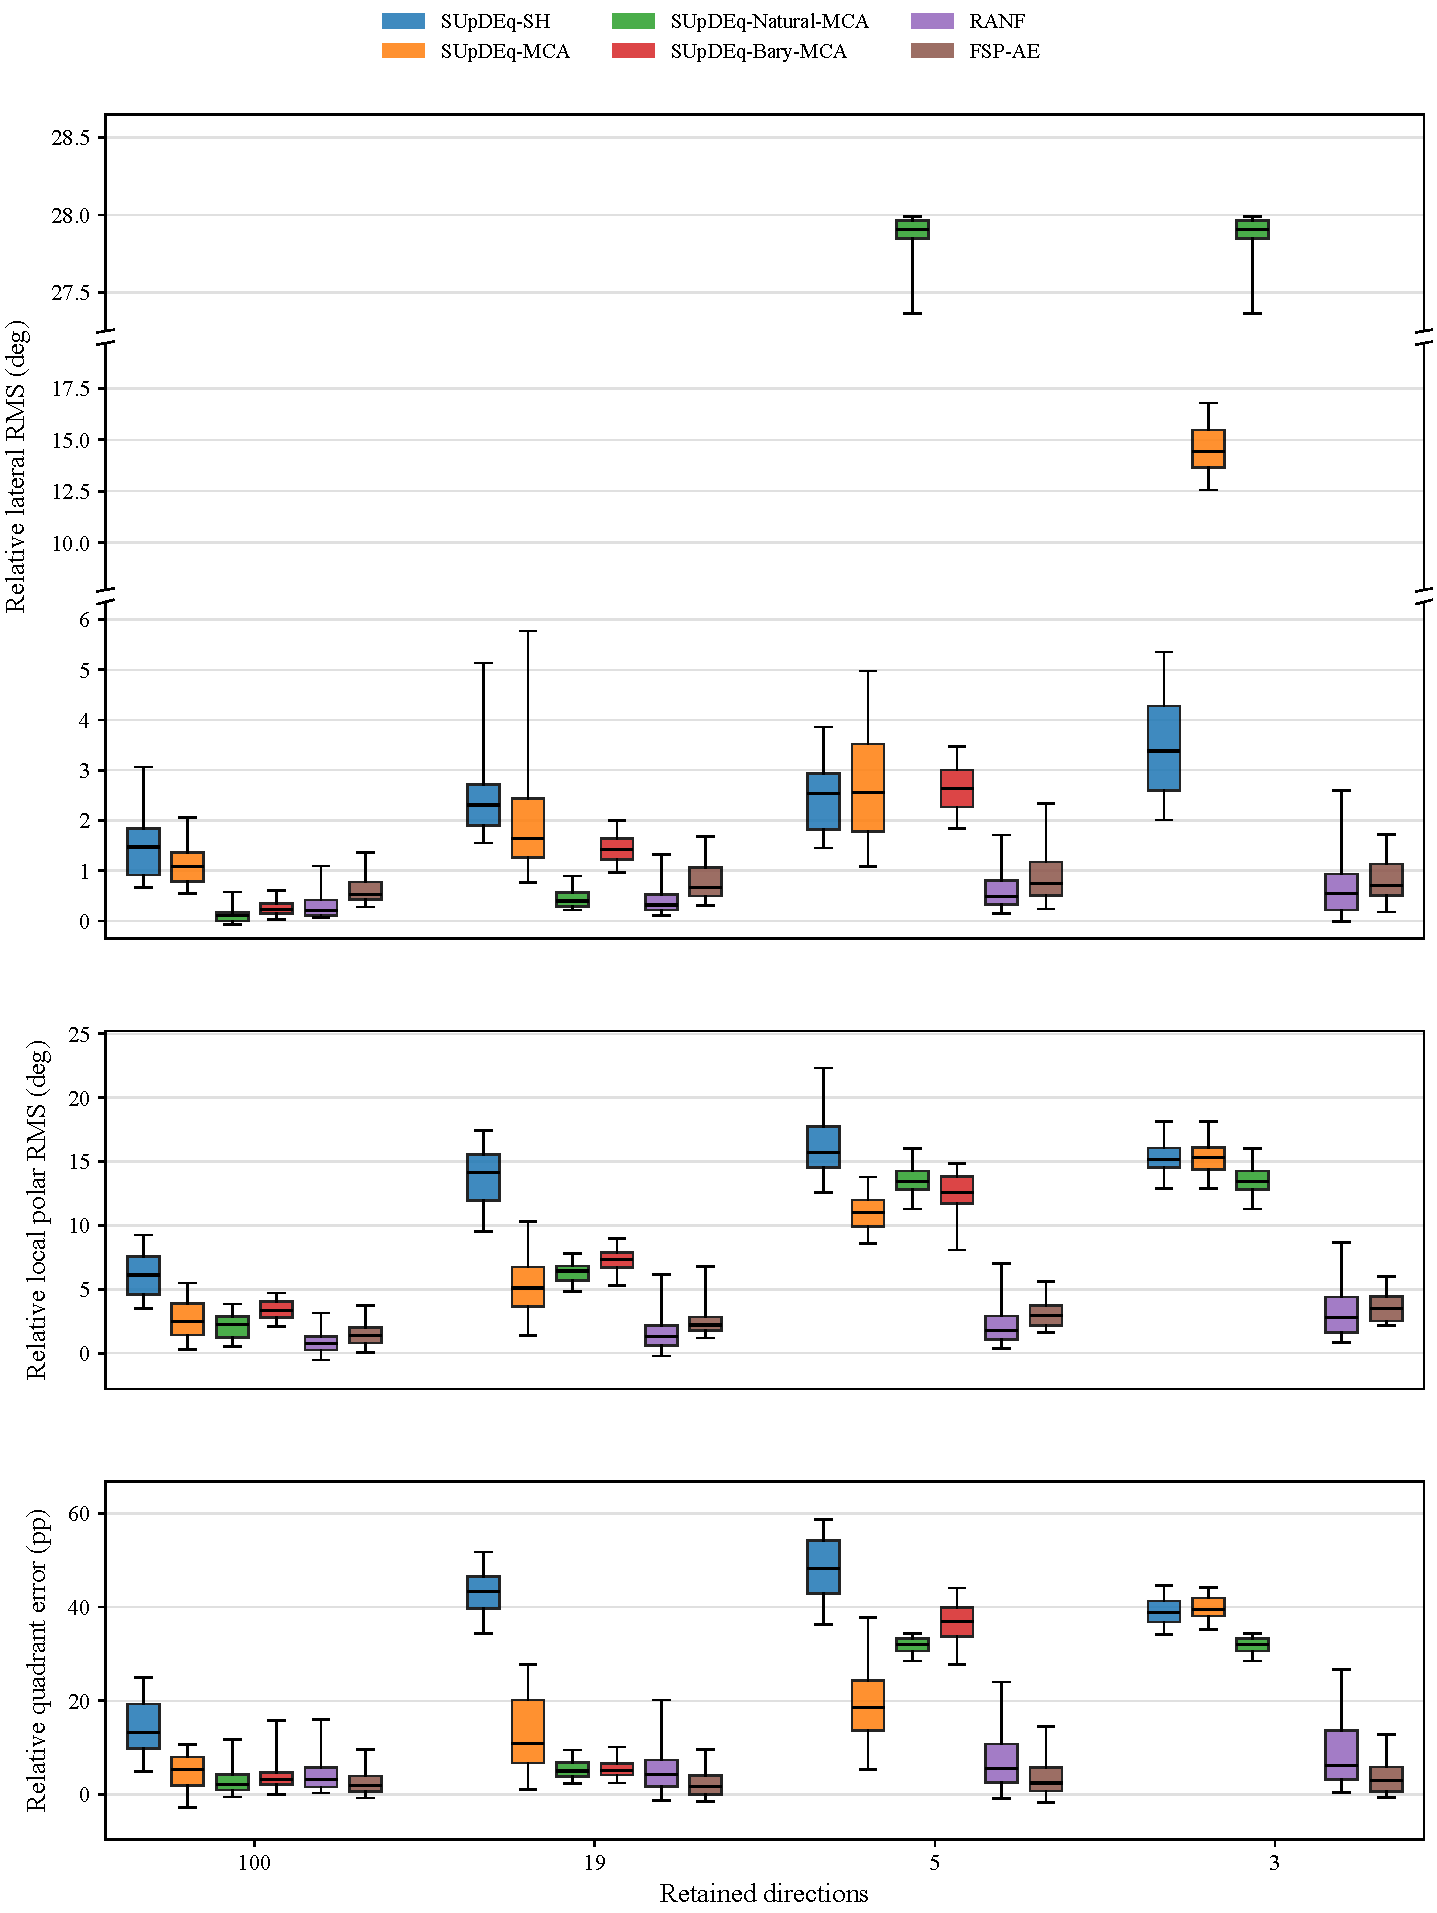
\includegraphics[width=\columnwidth]{figures/evaluation/bayesian_subject_boxplots.pdf}
    \caption[Subject-wise Bayesian-observer distribution summaries]{Subject-wise Bayesian-observer degradation over the 41 held-out subjects. Boxes show medians and interquartile ranges; whiskers span the 5th--95th percentiles. Metrics are relative to the dense self-reference condition, and the lateral RMS panel uses a broken vertical axis to show compact and high-error distributions together.}
    \label{fig:bayesian_subject_distributions}
\end{figure}

\subsection{Metric Relationships}
Figure~\ref{fig:metric_relationships} compares AIRM with conventional and Bayesian-observer summaries across the 943 completed rows. Because the rows form a repeated subject--method--condition design, inferential \(p\)-values are not computed by treating the rows as independent samples. Table~\ref{tab:metric_correlations} instead reports correlations over the 23 completed method--retention means, together with 95\% bootstrap intervals for the row-wise Spearman coefficients. Each of 1,000 bootstrap samples resamples subjects with replacement, retaining all method--condition results for each sampled subject. AIRM and LSD have a weak linear association but a strong rank association, indicating that the ordering of reconstruction quality is substantially shared even though the absolute scales are not linearly equivalent. AIRM is also strongly rank-associated with the Bayesian-observer summaries. The Fisher and Bayesian evaluations use the same cue families and related noise conventions, so this association shows consistency between two different analyses of shared model inputs rather than independent behavioural validation. These relationships are approximately monotonic, but they are not one-to-one. Several methods with similar LSD differ appreciably in AIRM, and some methods with comparable Bayesian localisation summaries differ in tensor discrepancy.

\begin{table}[!t]
\centering
\caption{Association between mean AIRM and established evaluation metrics. Correlations are computed over the 23 completed method--retention means; the final column gives a 95\% subject-cluster bootstrap interval for the corresponding row-wise Spearman coefficient.}
\label{tab:metric_correlations}
\scriptsize
\setlength{\tabcolsep}{2.0pt}
\resizebox{\columnwidth}{!}{%
\begin{tabular}{lrrr}
\toprule
Metric & Pearson $r$ & Spearman $\rho$ & Row-wise $\rho$ 95\% CI \\
\midrule
LSD & 0.25 & 0.86 & [0.82, 0.85] \\
ILD & 0.41 & 0.80 & [0.77, 0.80] \\
Relative lateral RMS & 0.97 & 0.95 & [0.86, 0.89] \\
Relative local polar RMS & 0.47 & 0.85 & [0.76, 0.81] \\
Relative quadrant error & 0.40 & 0.83 & [0.68, 0.73] \\
\bottomrule
\end{tabular}%
}
\end{table}


\begin{figure}[!htbp]
    \centering
    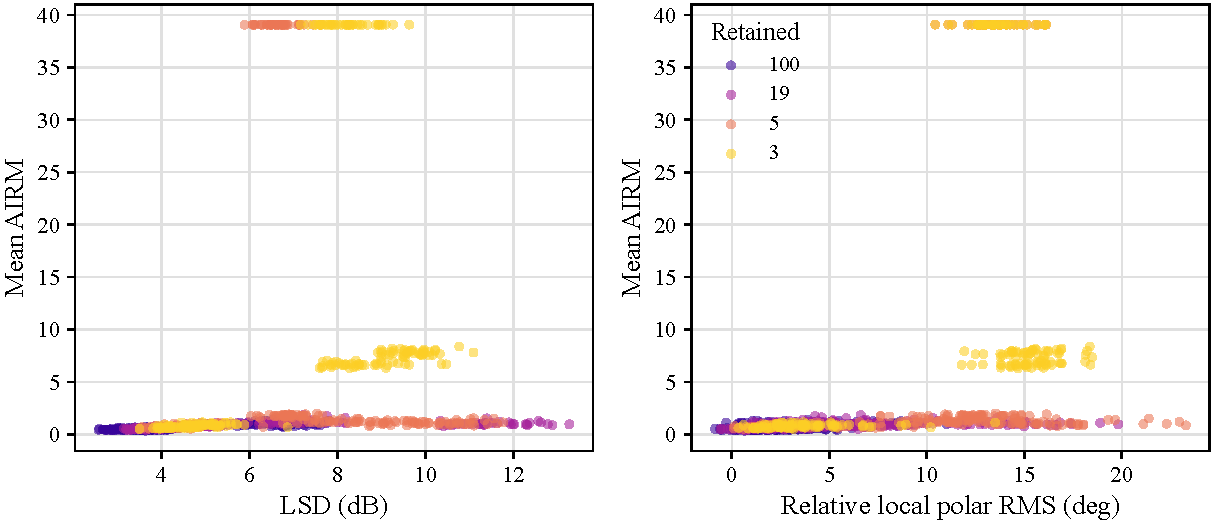
\includegraphics[width=\columnwidth]{figures/evaluation/metric_relationships_paper.pdf}
    \caption[Relationships between AIRM and other evaluation metrics]{Mean AIRM discrepancy against LSD and relative local polar RMS across completed subject--method--condition rows. Correlation summaries are reported in Table~\ref{tab:metric_correlations}.}
    \label{fig:metric_relationships}
\end{figure}

\subsection{Local Discrimination-Threshold Plausibility}
AIRM is a tensor distance, not itself an angular threshold. To express selected Fisher tensors in a more directly psychophysical unit, the \(d'=1\) threshold defined above was evaluated along lateral unit tangent directions at \((0^\circ,0^\circ)\), \((45^\circ,0^\circ)\), and \((90^\circ,0^\circ)\), and along vertical unit tangent directions at \((0^\circ,0^\circ)\) and \((0^\circ,45^\circ)\). Coordinate pairs denote azimuth and elevation. Values are converted from radians to degrees. Table~\ref{tab:local_threshold_plausibility} reports the resulting angular thresholds under the Barumerli/Reijniers cue-noise convention. These are derived from the same tensors as the ellipses in Fig.~\ref{fig:sonicom_kent}, without fitting to the behavioural minimum audible angles discussed below. Comparison with those measurements tests the plausibility of their scale and directional trend.

\begin{table}[!t]
\centering
\caption{Population-median Fisher-predicted local $d'=1$ angular thresholds in degrees. Lateral columns use horizontal-plane azimuthal displacements; vertical columns use frontal-plane elevational displacements.}
\label{tab:local_threshold_plausibility}
\scriptsize
\setlength{\tabcolsep}{2.4pt}
\resizebox{\columnwidth}{!}{%
\begin{tabular}{llrrrrrr}
\toprule
Method & $N$ & Lat. $(0,0)$ & Lat. $(45,0)$ & Lat. $(90,0)$ & Vert. $(0,0)$ & Vert. $(0,45)$ & Err. \\
\midrule
Measured & -- & 1.70 & 3.08 & 6.78 & 4.44 & 5.71 & 0.00 \\
SUpDEq-MCA & 19 & 1.84 & 2.55 & 5.66 & 4.27 & 5.00 & 0.54 \\
SUpDEq-MCA & 5 & 1.66 & 2.62 & 5.45 & 6.83 & 5.93 & 0.89 \\
SUpDEq-Bary-MCA & 19 & 1.83 & 3.02 & 5.77 & 6.31 & 7.04 & 0.88 \\
SUpDEq-Bary-MCA & 5 & 2.11 & 3.08 & 6.38 & 5.63 & 6.39 & 0.53 \\
RANF & 19 & 1.71 & 2.88 & 6.80 & 4.45 & 6.36 & 0.18 \\
RANF & 5 & 1.85 & 2.90 & 7.76 & 4.48 & 7.23 & 0.57 \\
FSP-AE & 19 & 1.81 & 3.32 & 7.76 & 4.72 & 6.53 & 0.49 \\
FSP-AE & 5 & 1.74 & 3.31 & 9.44 & 6.52 & 9.59 & 1.78 \\
\bottomrule
\end{tabular}%
}
\end{table}


The dense reference predicts increasing lateral thresholds from frontal to lateral directions, from \(1.70^\circ\) at \((0^\circ,0^\circ)\) to \(6.78^\circ\) at \((90^\circ,0^\circ)\). The vertical threshold increases from \(4.44^\circ\) at \((0^\circ,0^\circ)\) to \(5.71^\circ\) at \((0^\circ,45^\circ)\). This ordering is consistent with broadband spatial-resolution data: Stevenson-Hoare's Fig.~14 gives horizontal-plane means, collapsed over left and right, of approximately \(1.5^\circ\), \(2.7^\circ\), and \(7.2^\circ\) at \(0^\circ\), \(45^\circ\), and \(90^\circ\), respectively \cite{StevensonHoare2020}, while Grantham et al. report \(1.6^\circ\), \(2.8^\circ\), and \(6.5^\circ\) for horizontal, \(60^\circ\) diagonal, and vertical wideband-noise trajectories \cite{Grantham2003}. RANF preserves the five local thresholds most closely at \(N=19\); at \(N=5\), SUpDEq-Bary-MCA and RANF are closest. These local thresholds complement AIRM by showing how reconstruction changes predicted discrimination at specific directions.
\section{Discussion and Conclusion}

Bivariate Fisher information quantifies local discrimination from the spatial derivatives of the selected auditory cues under the assumed internal-noise model. AIRM measures reconstruction-induced changes in the scale, anisotropy, and orientation of these tensors. The Bayesian localisation model instead predicts pointing responses from sensory evidence, a prior, a decision rule, and response variability. The two analyses therefore assess predicted sensory discrimination and simulated pointing, respectively.

The high-sparsity results identify limits of the interpolation methods. Three retained directions do not satisfy the closed-hull requirement of SUpDEq-Bary-MCA, and SH-based or natural-neighbour interpolation can produce severe Fisher-tensor divergence at extreme sparsity even when conventional error summaries remain finite. RANF gives the strongest overall performance, while FSP-AE provides a second learning-based comparator with stable Fisher-tensor behaviour despite higher LSD.

The present Fisher analysis uses direction-independent cue-noise weights, so spatial variation in predicted discriminability arises from HRTF cue gradients rather than spatially varying internal noise. Allowing cue-noise covariance to vary with source direction would also account for direction-dependent sensory reliability. Such a model could distinguish the contributions of cue gradients and sensory reliability to predicted anisotropy. This extension is distinct from the equatorial prior in the Barumerli model: the prior biases point estimates towards more probable source regions, whereas direction-dependent cue noise would change the local discrimination threshold itself.

The Fisher tensor defines a direction-dependent metric on the sphere, so HRTF reconstruction can be viewed as preserving local cue derivatives rather than only matching spectra at sampled directions. A future learning objective could combine spectral error with an AIRM penalty on the reconstructed tensor field. A more tractable alternative may be to regularise the spatial Jacobians of PGE, ILD, and ITD directly. The neighbour-dissimilarity loss used in HRTFformer is related in purpose because it penalises local inconsistency across the reconstructed HRTF field rather than treating each direction as an isolated sample \cite{Hu2026HRTFformer}. The results show that preservation of local cue sensitivity provides a distinct criterion for HRTF reconstruction alongside spectral fidelity and predicted localisation error.

\FloatBarrier
\begingroup
\footnotesize
\setlength{\itemsep}{0pt}
\setlength{\parsep}{0pt}
\begin{thebibliography}{99}

\bibitem{Starch1905}
D. Starch, ``Perimetry of the localization of sound,'' \textit{Psychol. Rev. Monogr. Suppl.}, vol. 6, no. 4, pp. 1--45, 1905.

\bibitem{Carlile1997}
S. Carlile, P. Leong, and S. Hyams, ``The nature and distribution of errors in sound localization by human listeners,'' \textit{Hear. Res.}, vol. 114, nos. 1--2, pp. 179--196, 1997, doi:10.1016/S0378-5955(97)00161-5.

\bibitem{Barumerli2023}
R. Barumerli, P. Majdak, M. Geronazzo, D. Meijer, F. Avanzini, and R. Baumgartner, ``A Bayesian model for human directional localization of broadband static sound sources,'' \textit{Acta Acust.}, vol. 7, Art. no. 12, 2023, doi:10.1051/aacus/2023006.

\bibitem{Harper2004}
N. S. Harper and D. McAlpine, ``Optimal neural population coding of an auditory spatial cue,'' \textit{Nature}, vol. 430, no. 7000, pp. 682--686, 2004, doi:10.1038/nature02768.

\bibitem{Pavao2020}
R. Pav\~ao, E. S. Sussman, B. J. Fischer, and J. L. Pe\~na, ``Natural ITD statistics predict human auditory spatial perception,'' \textit{eLife}, vol. 9, Art. no. e51927, 2020, doi:10.7554/eLife.51927.

\bibitem{Dayan2001}
P. Dayan and L. F. Abbott, \textit{Theoretical Neuroscience}. Cambridge, MA, USA: MIT Press, 2001.

\bibitem{Rao1945}
C. R. Rao, ``Information and the accuracy attainable in the estimation of statistical parameters,'' \textit{Bull. Calcutta Math. Soc.}, vol. 37, no. 3, pp. 81--91, 1945.

\bibitem{Baumgartner2014}
R. Baumgartner, P. Majdak, and B. Laback, ``Modeling sound-source localization in sagittal planes for human listeners,'' \textit{J. Acoust. Soc. Am.}, vol. 136, no. 2, pp. 791--802, 2014, doi:10.1121/1.4887447.

\bibitem{Reijniers2014}
J. Reijniers, D. Vanderelst, C. Jin, S. Carlile, and H. Peremans,
``An ideal-observer model of human sound localization,''
\textit{Biol. Cybern.}, vol. 108, no. 2, pp. 169--181, 2014, doi:10.1007/s00422-014-0588-4.

\bibitem{Middlebrooks1999}
J. C. Middlebrooks, ``Virtual localization improved by scaling nonindividualized external-ear transfer functions in frequency,'' \textit{J. Acoust. Soc. Am.}, vol. 106, no. 3, pp. 1493--1510, 1999, doi:10.1121/1.427147.

\bibitem{Engel2023}
I. Engel \textit{et al.}, ``The SONICOM HRTF Dataset,'' \textit{J. Audio Eng. Soc.}, vol. 71, no. 5, pp. 241--253, 2023, doi:10.17743/jaes.2022.0066.

\bibitem{Hu2026HRTFformer}
X. Hu, J. Li, S. Zhang, S. Goetz, L. Picinali, O. B. Akan, and A. O. T. Hogg,
``HRTFformer: A Spatially-Aware Transformer for Individual HRTF Upsampling in Immersive Audio Rendering,''
arXiv:2510.01891, 2026, doi:10.48550/arXiv.2510.01891.

\bibitem{Hogg2025LAPUpsampling}
A. O. T. Hogg, R. Barumerli, R. Daugintis, K. C. Poole, F. Brinkmann, L. Picinali, and M. Geronazzo,
``Listener Acoustic Personalization Challenge--LAP24: Head-Related Transfer Function Upsampling,''
\textit{IEEE Open J. Signal Process.}, vol. 6, pp. 926--941, 2025, doi:10.1109/OJSP.2025.3588776.


\bibitem{Poerschmann2019SUpDEq}
C. P\"orschmann, J. M. Arend, and F. Brinkmann, ``Directional Equalization of Sparse Head-Related Transfer Function Sets for Spatial Upsampling,'' \textit{IEEE/ACM Trans. Audio Speech Lang. Process.}, vol. 27, no. 6, pp. 1060--1071, 2019, doi:10.1109/TASLP.2019.2908057.

\bibitem{Masuyama2025RANF}
Y. Masuyama, G. Wichern, F. G. Germain, C. Ick, and J. Le Roux,
``RANF: Neural field-based HRTF spatial upsampling with retrieval augmentation and parameter efficient fine-tuning,''
\textit{IEEE Open J. Signal Process.}, vol. 7, pp. 32--41, 2026, doi:10.1109/OJSP.2025.3640517.

\bibitem{Masuyama2025ICASSPRANF}
Y. Masuyama, G. Wichern, F. G. Germain, C. Ick, and J. Le Roux,
``Retrieval-Augmented Neural Field for HRTF Upsampling and Personalization,''
in \textit{Proc. IEEE Int. Conf. Acoust., Speech Signal Process. (ICASSP)}, 2025, pp. 1--5, doi:10.1109/ICASSP49660.2025.10889481.

\bibitem{Ito2025FSPAE}
Y. Ito, T. Nakamura, S. Koyama, S. Sakamoto, and H. Saruwatari,
``Spatial Upsampling of Head-Related Transfer Function Using Neural Network Conditioned on Source Position and Frequency,''
\textit{IEEE Open J. Signal Process.}, vol. 6, pp. 1109--1123, 2025, doi:10.1109/OJSP.2025.3613132.

\bibitem{StevensonHoare2020}
J. O. Stevenson-Hoare, \textit{Auditory Spatial Precision in the Horizontal Plane}, Ph.D. dissertation, School of Psychology, Cardiff University, 2020.

\bibitem{Grantham2003}
D. W. Grantham, B. W. Y. Hornsby, and E. A. Erpenbeck, ``Auditory spatial resolution in horizontal, vertical, and diagonal planes,'' \textit{J. Acoust. Soc. Am.}, vol. 114, no. 2, pp. 1009--1022, 2003, doi:10.1121/1.1590970.

\end{thebibliography}
\endgroup

\section*{Author Biographies}

\begin{center}
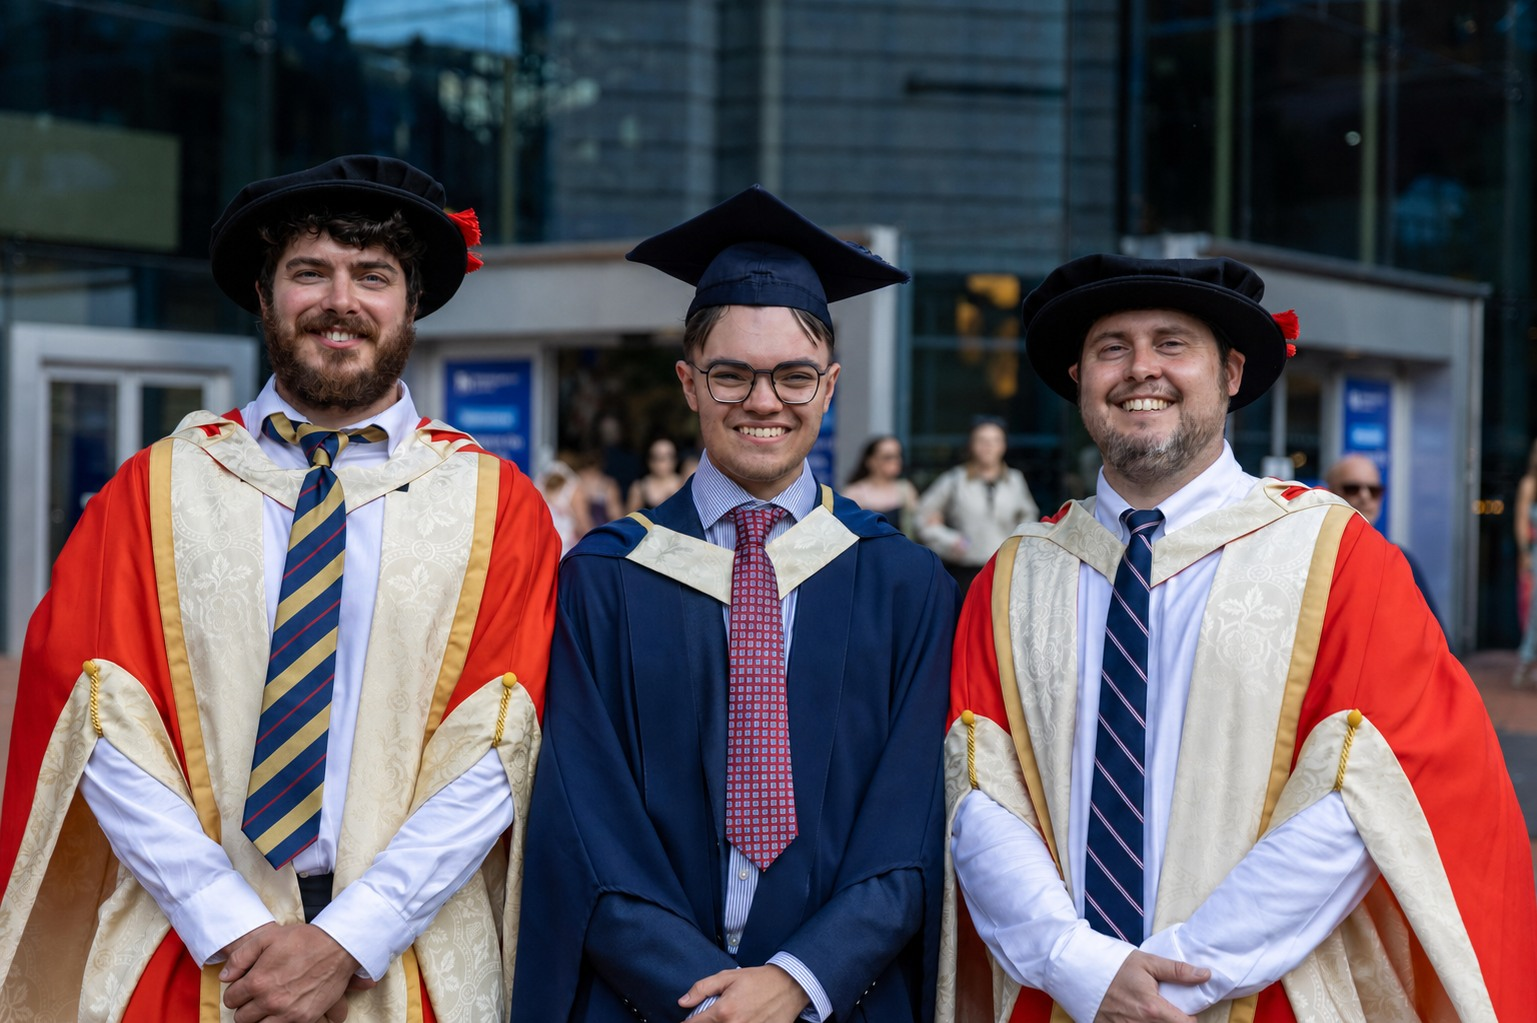
\includegraphics[width=\columnwidth]{figures/authors_cheshire_bassett_smith.jpg}\\[-0.2em]
{\footnotesize\itshape Left to right: Matthew Cheshire, Dominic Bassett, and Samuel Smith.}
\end{center}

\begingroup
\setlength{\parskip}{0pt}

\noindent\textbf{Dominic Bassett} received the B.Sc. (Hons.) degree in Sound Engineering and Production with first-class honours from Birmingham City University, Birmingham, U.K., in 2026. His dissertation investigated statistical methods for modelling spatial acuity in head-related transfer function upsampling. He is a Graduate Acoustic Consultant with Cundall. His interests include spatial audio signal processing, room-acoustic simulation, and perceptual modelling. He has contributed to open-source acoustical modelling software, including work on binaural auralisation tools.

\vspace{0.4em}
\newpage

\noindent\textbf{Matthew Cheshire} is a Lecturer in Audio Engineering in the College of Computing at Birmingham City University, Birmingham, U.K., where he leads modules in audio embedded systems, music information retrieval, and live sound reinforcement. He received the B.Sc. (Hons.) degree in Sound Engineering and Production from Birmingham City University in 2013 and the Ph.D. degree from the same institution in 2023. His doctoral research investigated timbral analysis and recording-parameter transformations of snare drums. His research interests include microphone comparison, drum recording, perceptual evaluation, and signal processing for recording applications. He has authored papers presented at Audio Engineering Society conventions and published in the \textit{Journal of the Audio Engineering Society}. He received the AES Saul Walker Award in 2019 and the AES Educational Foundation John Eargle Award in 2020 and 2021.

\vspace{0.4em}

\noindent\textbf{Samuel Smith} is a Senior Lecturer in the College of Computing at Birmingham City University, Birmingham, U.K., where he leads modules in digital signal processing, digital audio effects, and audio and video processing. He received the B.Sc. (Hons.) degree in Sound Engineering and Production from Birmingham City University in 2012 and the Ph.D. degree from the same institution in 2021. His doctoral research developed a statistical approach for three-dimensional surface detection. His research interests include audio signal processing, music information retrieval, medical image processing, and computer vision. He has authored papers in \textit{IEEE Signal Processing Letters} and \textit{Transactions of the International Society for Music Information Retrieval}, and has co-authored work presented at Audio Engineering Society conferences.
\endgroup

\end{document}

